\section{Cloudsysteme -- Funktionalität}
\label{sec:cloudfunktionalitaet}

\textbf{Was ändert sich in der Cloud?}
\begin{items}
	\item Physischer Entwurf muss automatisch erfolgen
	\item Obligatorische Datenverteilung
	\item Anfrageauswertung in Gegenwart anderer Anfragen
		\\*
		\( \leadsto \) entsprechende Planung
	\item Unterschiedliche QoS-Vereinbarungen mit unterschiedlichen Dienstnehmern
	\item Plötzliche extreme Zunahme von Zugriffen eines Dienstnehmers i.A. nicht vorhersehbar 
		\\*
		\( \leadsto \) Infrastruktur sollte damit umgehen können
	\item \emph{Secure Storage}: Verschlüsselung der Daten, trotzdem soll Dienstanbieter möglichst großen Teil der Anfrageauswertung übernehmen
\end{items}

\textbf{Relationale Algebra}
\begin{items}
	\item \underline{Projektion}: Optimierung: bei vielen Projektionen hintereinander reicht die zuletzt ausgeführte auch allein:
		\\*
		\( \pi \)\lstinline{[KName](}\( \pi \)\lstinline{[KName, Land](Kuenstler))} \( \leadsto \) \( \pi \)\lstinline{[KName](Kuenstler)}
	\item \underline{Selektion}: Optimierung: Selektionen lassen sich beliebig vertauschen, manchmal auch Projektion und Selektion
	\item \underline{Verbund}: Kommutativ, Assoziativ
		\\*
		Nested-Loop Join: Teuer, da pro Eintrag links über alle rechten Einträge iteriert wird
		\\*
		Merge Join: Beide Relationen sortieren, dann Eintrag für Eintrag
\end{items}

\textbf{Blockierende/Nichtblockierende Operatoren}
\begin{items}
	\item Operator blockiert \( \Leftrightarrow \) Ergebnis des Operators muss vor Ausführung des nachfolgenden vollständig berechnet sein \\* (z.B. Sort-Operator)
\end{items}

\textbf{Histogramme}
\begin{items}
	\item Zeigt Auftrittshäufigkeit eines Intervalls
	\item \underline{Equi-Width-Histogramm}: Breite aller Buckets gleich
	\item \underline{Equi-Depth-Histogramm}: Auftrittshäufigkeit aller Buckets gleich
	\item Nützlich bei ein-Attribut-Anfragen, sonst nicht so:
		\\*
		Mehrdimensionale Histogramme schwer konstruierbar und wartbar, Anzahl Attributkombinationen exponentiell wachsend zur Anzahl der Attribute
\end{items}

\textbf{Synchroner und asynchroner Zugriff}
\begin{items}
	\item \underline{Synchron}: innerhalb einer Transaktion
	\item \underline{Asynchron}: mehrere Transaktionen
\end{items}

\textbf{Service-Level Agreements}
\begin{items}
	\item Vereinbarung zwischen Client und Server bzgl. Dienstausführung
		\\*
		``Antwort innserhalb von 300ms für 99,9\% der Aufrufe bei 500 Zugriffen pro Sekunde''
\end{items}

\textbf{Zustände}
\begin{items}
	\item \underline{Zustandslos}: z.B. Umrechnungsdienst
	\item \underline{Zustandsbehaftet}: z.B. Ausführung Geschäftsprozess
\end{items}

\textbf{Quorum}
\begin{items}
	\item Szenario: Replikation mit \( n \) Knoten
		\\*
		\( \leadsto \) Wie Konsistenz sicherstellen? Was, wenn nicht alle Knoten verfügbar?
	\item \underline{Quorum Consensus}:
		\\*
		Lesen: Lese Mindestanzahl von Versionen (\( R \)), nehme aktuelle
		\\*
		Schreiben: Aktualisiere Mindestanzahl von Kopien (\( W \))
\end{items}

\newpage

\textbf{P2P}
\begin{items}
	\item \emph{peer to peer}-Systeme:
		\\*
		Jeder Knoten für Ausschnitt des Schlüsselraums verantwortlich
		\\*
		Verwaltung von (Schlüssel, Wert)-Paaren
		\\*
		(put, get)-Interface
		\\*
		Zu Größe des Schlüsselraums logarithmischer Suchaufwand
	\item Beispiel: Chord
		\\*
		Zentrale Datenstruktur: \emph{identifier circle}, \emph{chord ring}
		\\* Suche: Jeder Knoten hat \emph{finger table}, \emph{i}-ter Eintrag von Knoten \( n \): successor(\( n+2^{i-1} \)) (\( m \) Anzahl Bits)
	\begin{figure}[H]\centering\label{Chord}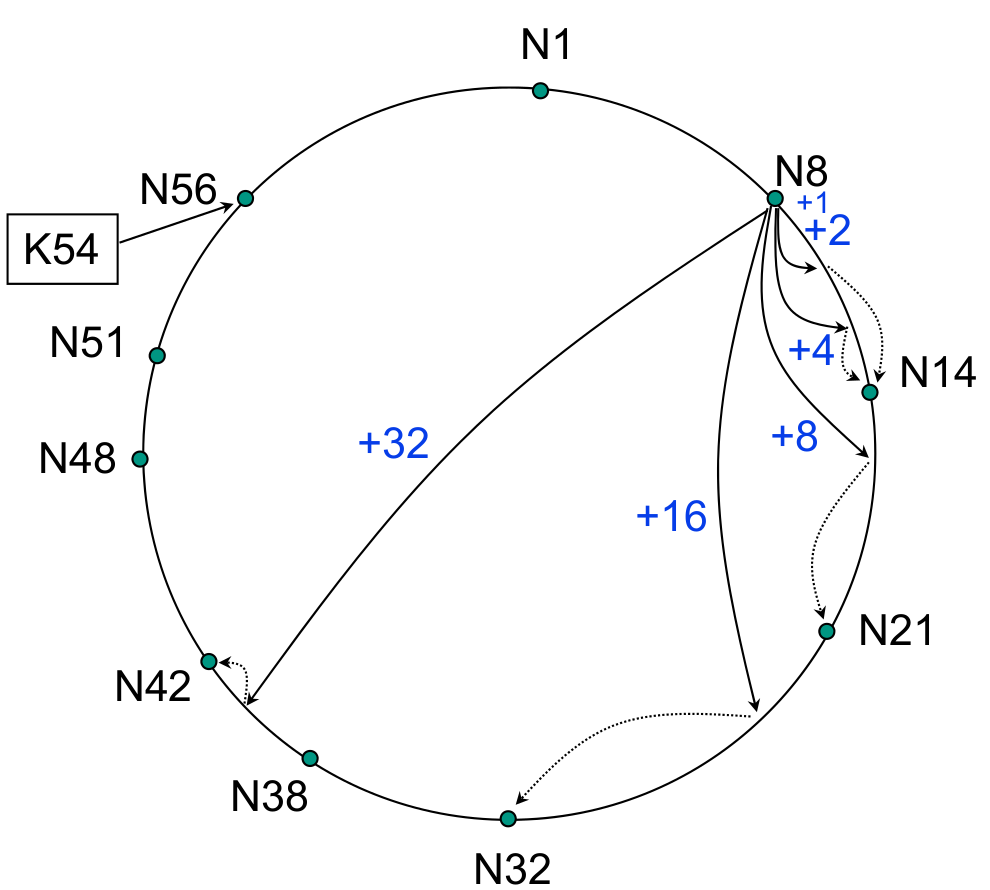
\includegraphics[width=0.25\textwidth]{Chord}\end{figure}
	\item Replikation über \emph{chained replication}: Schlüssel nicht nur bei einem Knoten, sondern auch bei \( k \) Nachfolgern einfügen
	\item \underline{Heterogenität}: Knoten können unterschiedlich leistungsstark sein (ggf. unterschiedliche Zuständigkeitsbereiche, unterschiedliche Last)
\end{items}

\textbf{Dynamo}
\begin{items}
	\item Key-Value-Store
	\item get-/put-Interface
	\item Objekte BLOBs \( \leadsto \) kein DB-Schema \( \leadsto \) Interpretieren nötig
	\item Keine Isolation \( \leadsto \) keine totale Konsistenz
	\item Schreibzugriff jeweils nur für ein Objekt
\end{items}
\begin{figure}[H]\centering\label{UebersichtDynamo}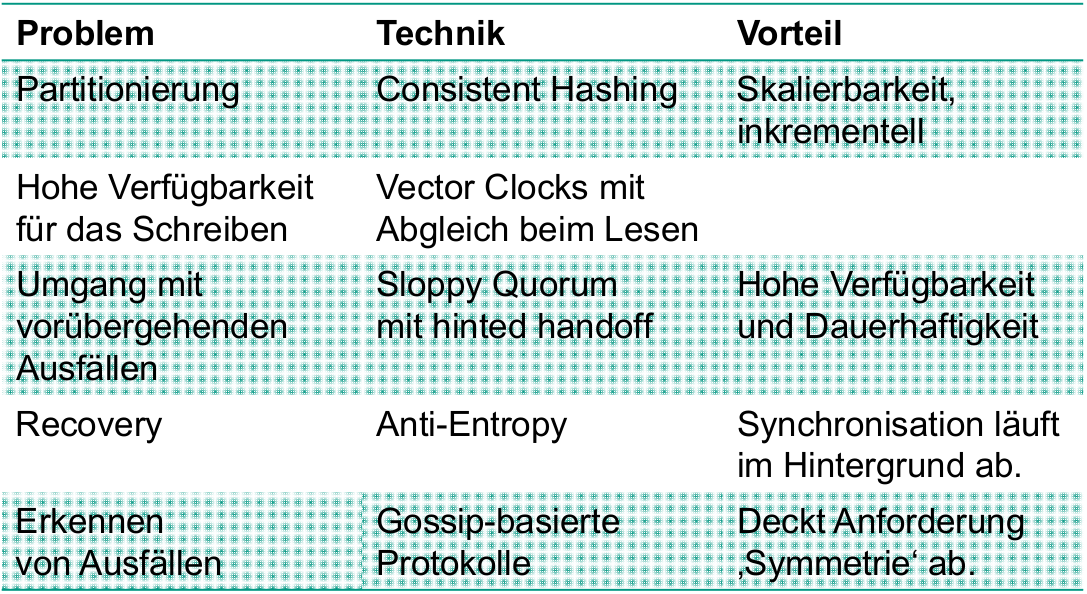
\includegraphics[width=0.33\textwidth]{UebersichtDynamo}\end{figure}

\textbf{Dynamo -- Vector Clocks}
\begin{items}
	\item Ziel: eventual consistency
	\item Liste von (Knoten, Zähler)-Paaren (eine Liste pro Version) \( \leadsto \) Erfassung der Zusammenhönge zwischen Versionen
	\item Quorum-basierte Techniken \( \leadsto \) Inkonsistenzen vermeiden
	\item vector clock-basierte Techniken \( \leadsto \) Inkonsistenzen erkennen und auflösen
\end{items}